% !TEX TS-program = pdfLaTeX+shellescape
% !TEX encoding = UTF-8 Unicode

\documentclass[class=beamer,tikz]{standalone}
\setbeamertemplate{navigation symbols}{} % For delete the navigation symbols
\usefonttheme{professionalfonts}
\usepackage{luatexja}
% \usepackage{pgfplots}
% \pgfplotsset{compat=1.17}

\usepackage{colortbl,array,xcolor}
\usepackage{amsmath,amsfonts}
\usepackage{bm}

\begin{document}
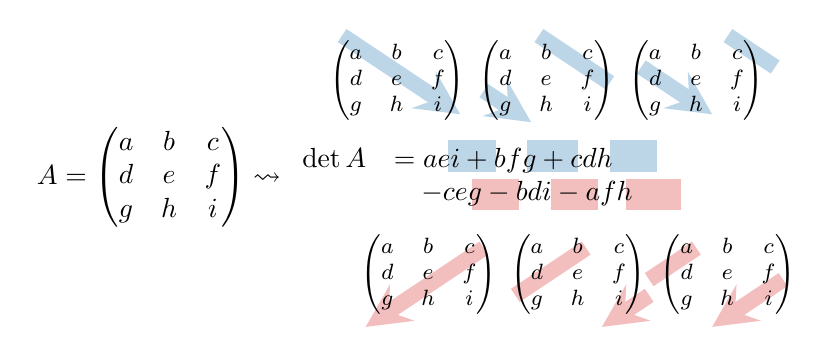
\begin{tikzpicture}
    \definecolor{tab_red}{HTML}{d62728}
    \definecolor{tab_blue}{HTML}{1f77b4}
    \definecolor{tab_green}{HTML}{2ca02c}
    \definecolor{tab_brown}{HTML}{8c564b}
    %\draw[help lines] (0,0) grid (14,6);

    \draw[color=tab_blue!30, line width=4.0mm] (6.35,3.27) -- (6.95,3.27);
    \draw[color=tab_blue!30, line width=4.0mm] (7.35,3.27) -- (8.00,3.27);
    \draw[color=tab_blue!30, line width=4.0mm] (8.40,3.27) -- (9.00,3.27);
    \draw[color=tab_red!30, line width=4.0mm] (6.65,2.78) -- (7.25,2.78);
    \draw[color=tab_red!30, line width=4.0mm] (7.65,2.78) -- (8.25,2.78);
    \draw[color=tab_red!30, line width=4.0mm] (8.60,2.78) -- (9.30,2.78);
    
    \draw[-stealth, color=tab_blue!30, line width=2.0mm] (5.0,4.8) -- (6.5,3.8);
    \draw[color=tab_blue!30, line width=2.0mm] (7.5,4.8) -- (8.4,4.2);
    \draw[-stealth, color=tab_blue!30, line width=2.0mm] (6.8,4.1) -- (7.4,3.7);
    \draw[color=tab_blue!30, line width=2.0mm] (9.9,4.8) -- (10.5,4.4);
    \draw[-stealth, color=tab_blue!30, line width=2.0mm] (8.8,4.4) -- (9.7,3.8);
    
    \draw[-stealth, color=tab_red!30, line width=2.0mm] (6.8,2.1) -- (5.3,1.1);
    \draw[color=tab_red!30, line width=2.0mm] (8.1,2.1) -- (7.2,1.5);
    \draw[-stealth, color=tab_red!30, line width=2.0mm] (8.9,1.5) -- (8.3,1.1);
    \draw[color=tab_red!30, line width=2.0mm] (9.5,2.1) -- (8.9,1.7);
    \draw[-stealth, color=tab_red!30, line width=2.0mm] (10.6,1.7) -- (9.7,1.1);
    

    % \draw[color=tab_blue!30, line width=2.0mm] (5.3,4.8) -- (6.3,4.05) arc (50:-130:0.45) -- (4.8,4.00);
    % \draw[color=tab_blue!30, line width=2.0mm] (6.1,4.6) -- (5.3,5.15) arc (50:240:0.45) -- (5.55,3.85);
    

    \node[anchor=west] (matrix) at (1,3.0) {
        $A = \begin{pmatrix} 
            a & b & c \cr 
            d & e & f \cr 
            g & h & i 
        \end{pmatrix} \leadsto \begin{array}{rl}\det A &= aei + bfg + cdh \cr &\quad -ceg - bdi - afh\end{array}$
    };
    \node[anchor=south] (matrix1) at (5.70, 3.60) {
        \footnotesize$\begin{pmatrix} 
            a & b & c \cr 
            d & e & f \cr 
            g & h & i 
        \end{pmatrix}$
    };
    \node[anchor=south] (matrix2) at (7.60, 3.60) {
        \footnotesize$\begin{pmatrix} 
            a & b & c \cr 
            d & e & f \cr 
            g & h & i 
        \end{pmatrix}$
    };
    \node[anchor=south] (matrix3) at (9.50, 3.60) {
        \footnotesize$\begin{pmatrix} 
            a & b & c \cr 
            d & e & f \cr 
            g & h & i 
        \end{pmatrix}$
    };
    \node[anchor=north] (matrix4) at (6.10, 2.40) {
        \footnotesize$\begin{pmatrix} 
            a & b & c \cr 
            d & e & f \cr 
            g & h & i 
        \end{pmatrix}$
    };
    \node[anchor=north] (matrix5) at (8.00, 2.40) {
        \footnotesize$\begin{pmatrix} 
            a & b & c \cr 
            d & e & f \cr 
            g & h & i 
        \end{pmatrix}$
    };
    \node[anchor=north] (matrix6) at (9.90, 2.40) {
        \footnotesize$\begin{pmatrix} 
            a & b & c \cr 
            d & e & f \cr 
            g & h & i 
        \end{pmatrix}$
    };
    
    
\end{tikzpicture}
\end{document}